% vim:tw=72 sw=2 ft=tex
%         File: HW2.tex
% Date Created: 2016 Feb 11
%  Last Change: 2016 Feb 21
%     Compiler: pdflatex
%       Author: Adam Lang $ Gabriel Anderson Santiago
\documentclass[12pt,a4paper]{article}
\usepackage{amsmath, amssymb}
\usepackage[utf8]{inputenc}
\usepackage[T1]{fontenc}
\usepackage[english]{babel}
\usepackage{graphicx}
\usepackage{float}
\graphicspath{{fig/}}
\usepackage{tikz}

\title{Homework assignment 2 - EL2450}
\author{Adam Lang (861110-3956) \& Gabriel Andersson Santiago
(910706-4538)}

\begin{document}
\maketitle
\section{Rate Monotonic} %1
\subsection{}
  Rate Monotonic scheduling is a scheduling method that will
  predetermine the priority of each task proportional to the tasks
  activation frequency. The priority is determined at the task creation
  and will remain unchanged during the whole application.

\subsection{} %2
  A set of tasks $J=\{J_1,J_2,...,J_n\}$ is schedulable with RM if
  \begin{equation}
    U=\sum\limits_{i=1}^n \frac{C_i}{T_i} \leq n(2^{1/n}-1)
  \end{equation}
  where $C_i$ is the computation time, $T_i$ is the period, $U$ is the
  utilization factor and $n$ is the
  number of computations. When we have a sampling time of 
  $T=\{20, 29, 30\}ms$ and a computation time of 6 ms each we can see that,
  \begin{equation}
    \frac{6}{20}+\frac{6}{29}+\frac{6}{35}=0.678
  \end{equation}
  and with a utilization factor of $U = 0.780$ we can see that the set
  of tasks $J$ should be schedulable with RM.

\subsection{}%3
 The pendulums are indeed stabilized. There is however a slight
 difference in the control performance. From what we can see is the
 settling time longer the shorter the pendulum gets. Which is correct
 according to the lab    	introduction. 
  \begin{center}
      \begin{figure}[H]
      \centering
        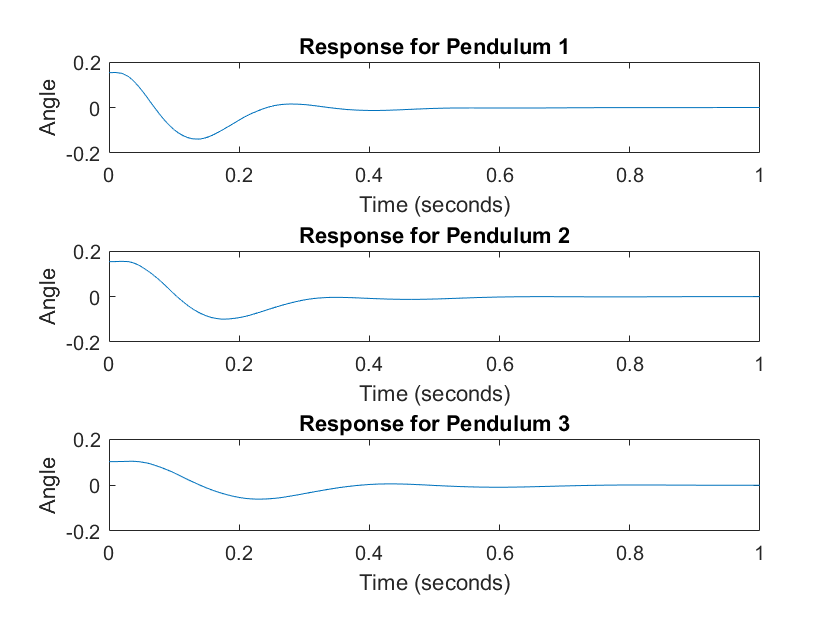
\includegraphics[scale=0.5]{ex31.png}
        \caption{Pendulum angles for the three different pendulums}
        \label{fig:ex31}
      \end{figure}
    \end{center}
    
    \begin{center}
      \begin{figure}[H]
      \centering
        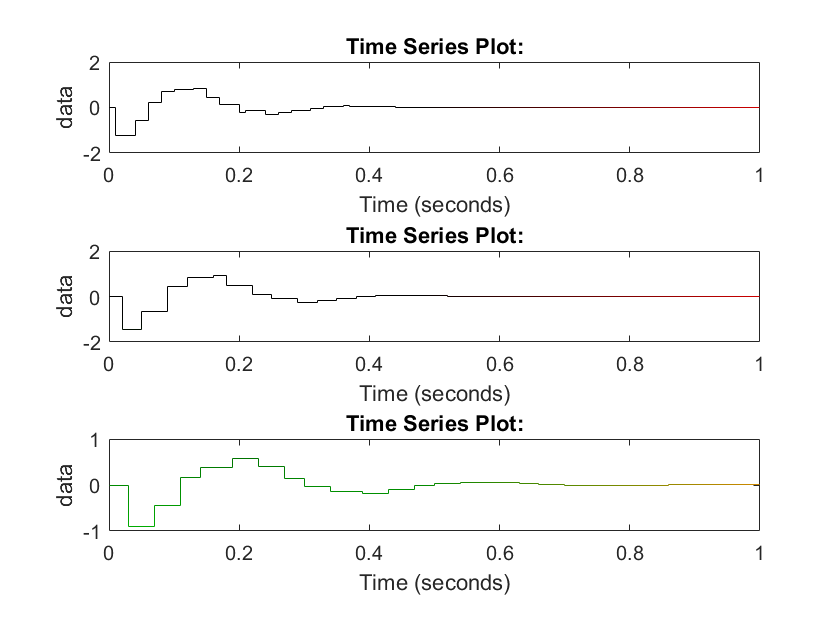
\includegraphics[scale=0.5]{ex32.png}
      \caption{Control signal for pendulum}
        \label{fig:ex32}
      \end{figure}
    \end{center}

   

\subsection{}%4

The schedule plot from Simulink corresponds to our own schedule. This
can be seen in figure 3 and 4. Be aware that our schedule is ordered
from shortest-longest pendulum and the one from Simulink is
longest-shortest pendulum.
    \begin{center}
      \begin{figure}[H]
      \centering
        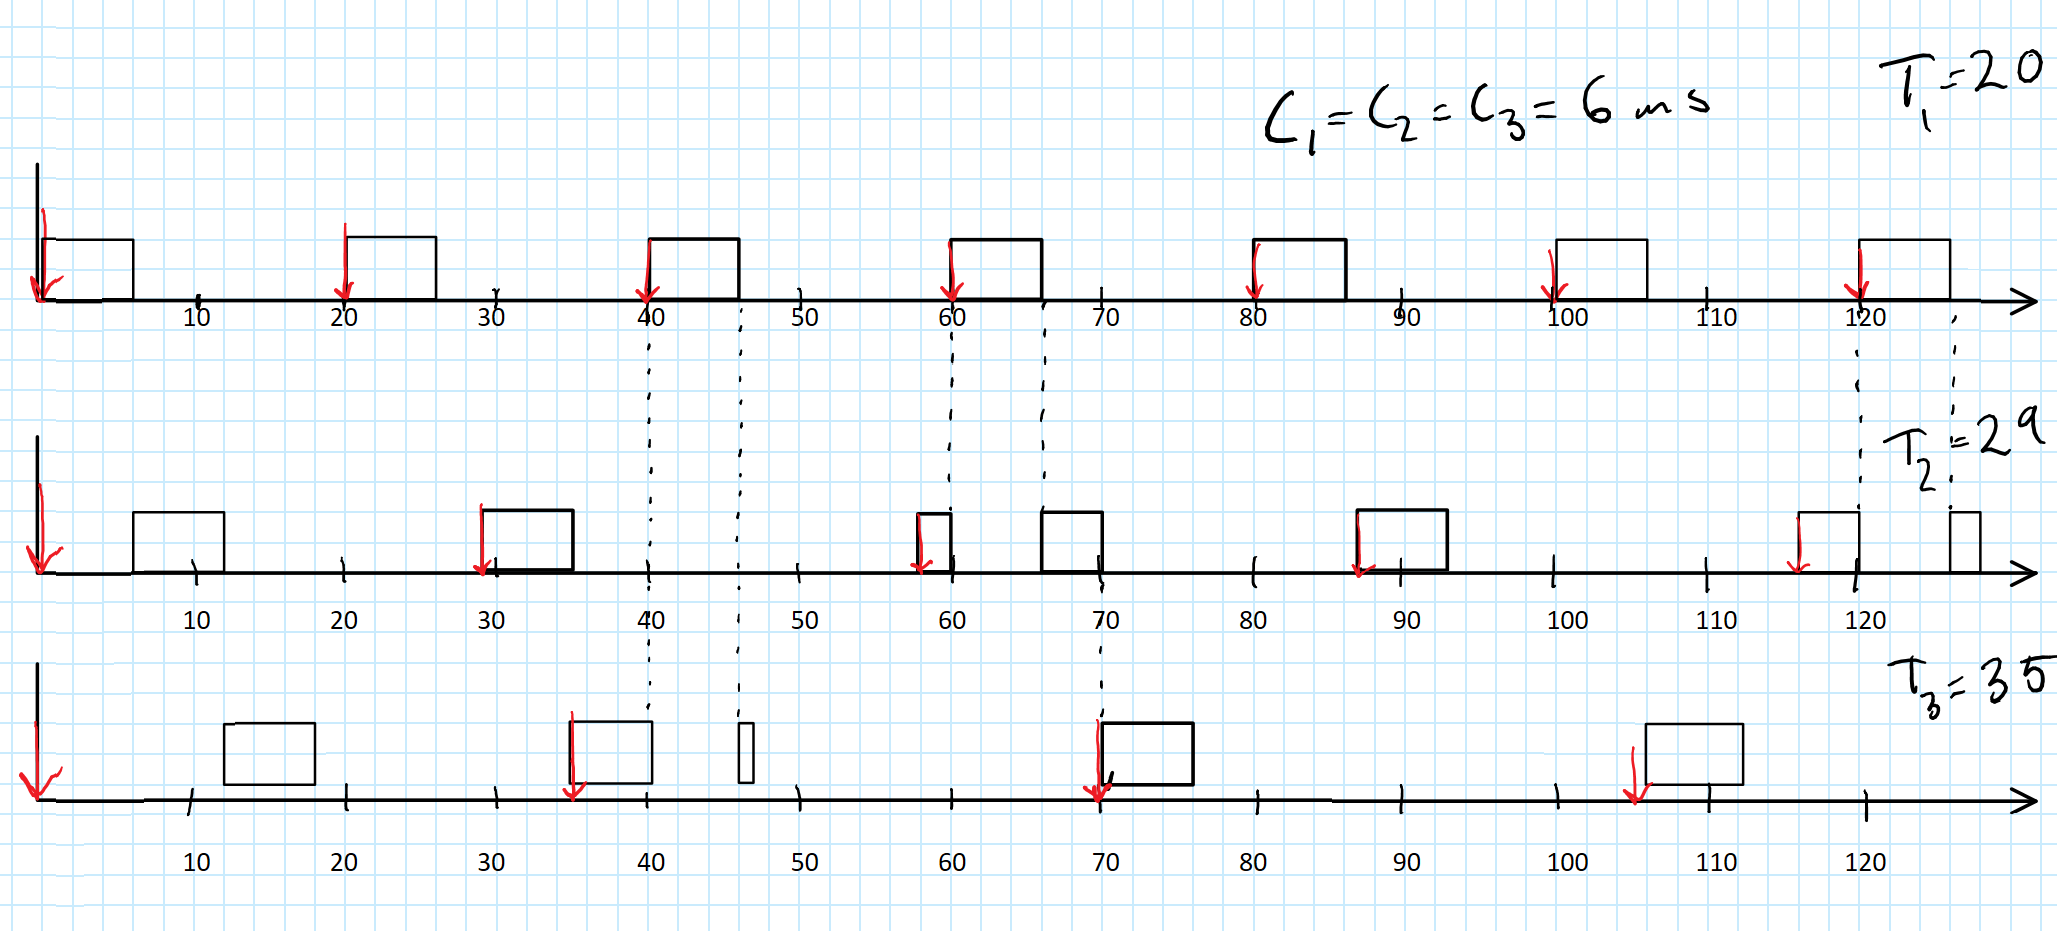
\includegraphics[scale=0.3]{ex41.png}
        \caption{Our schedule for 6 ms computation time}
        \label{fig:ex41}
     \end{figure}
    \end{center}
    
    \begin{center}
     \begin{figure}[H]
      \centering
        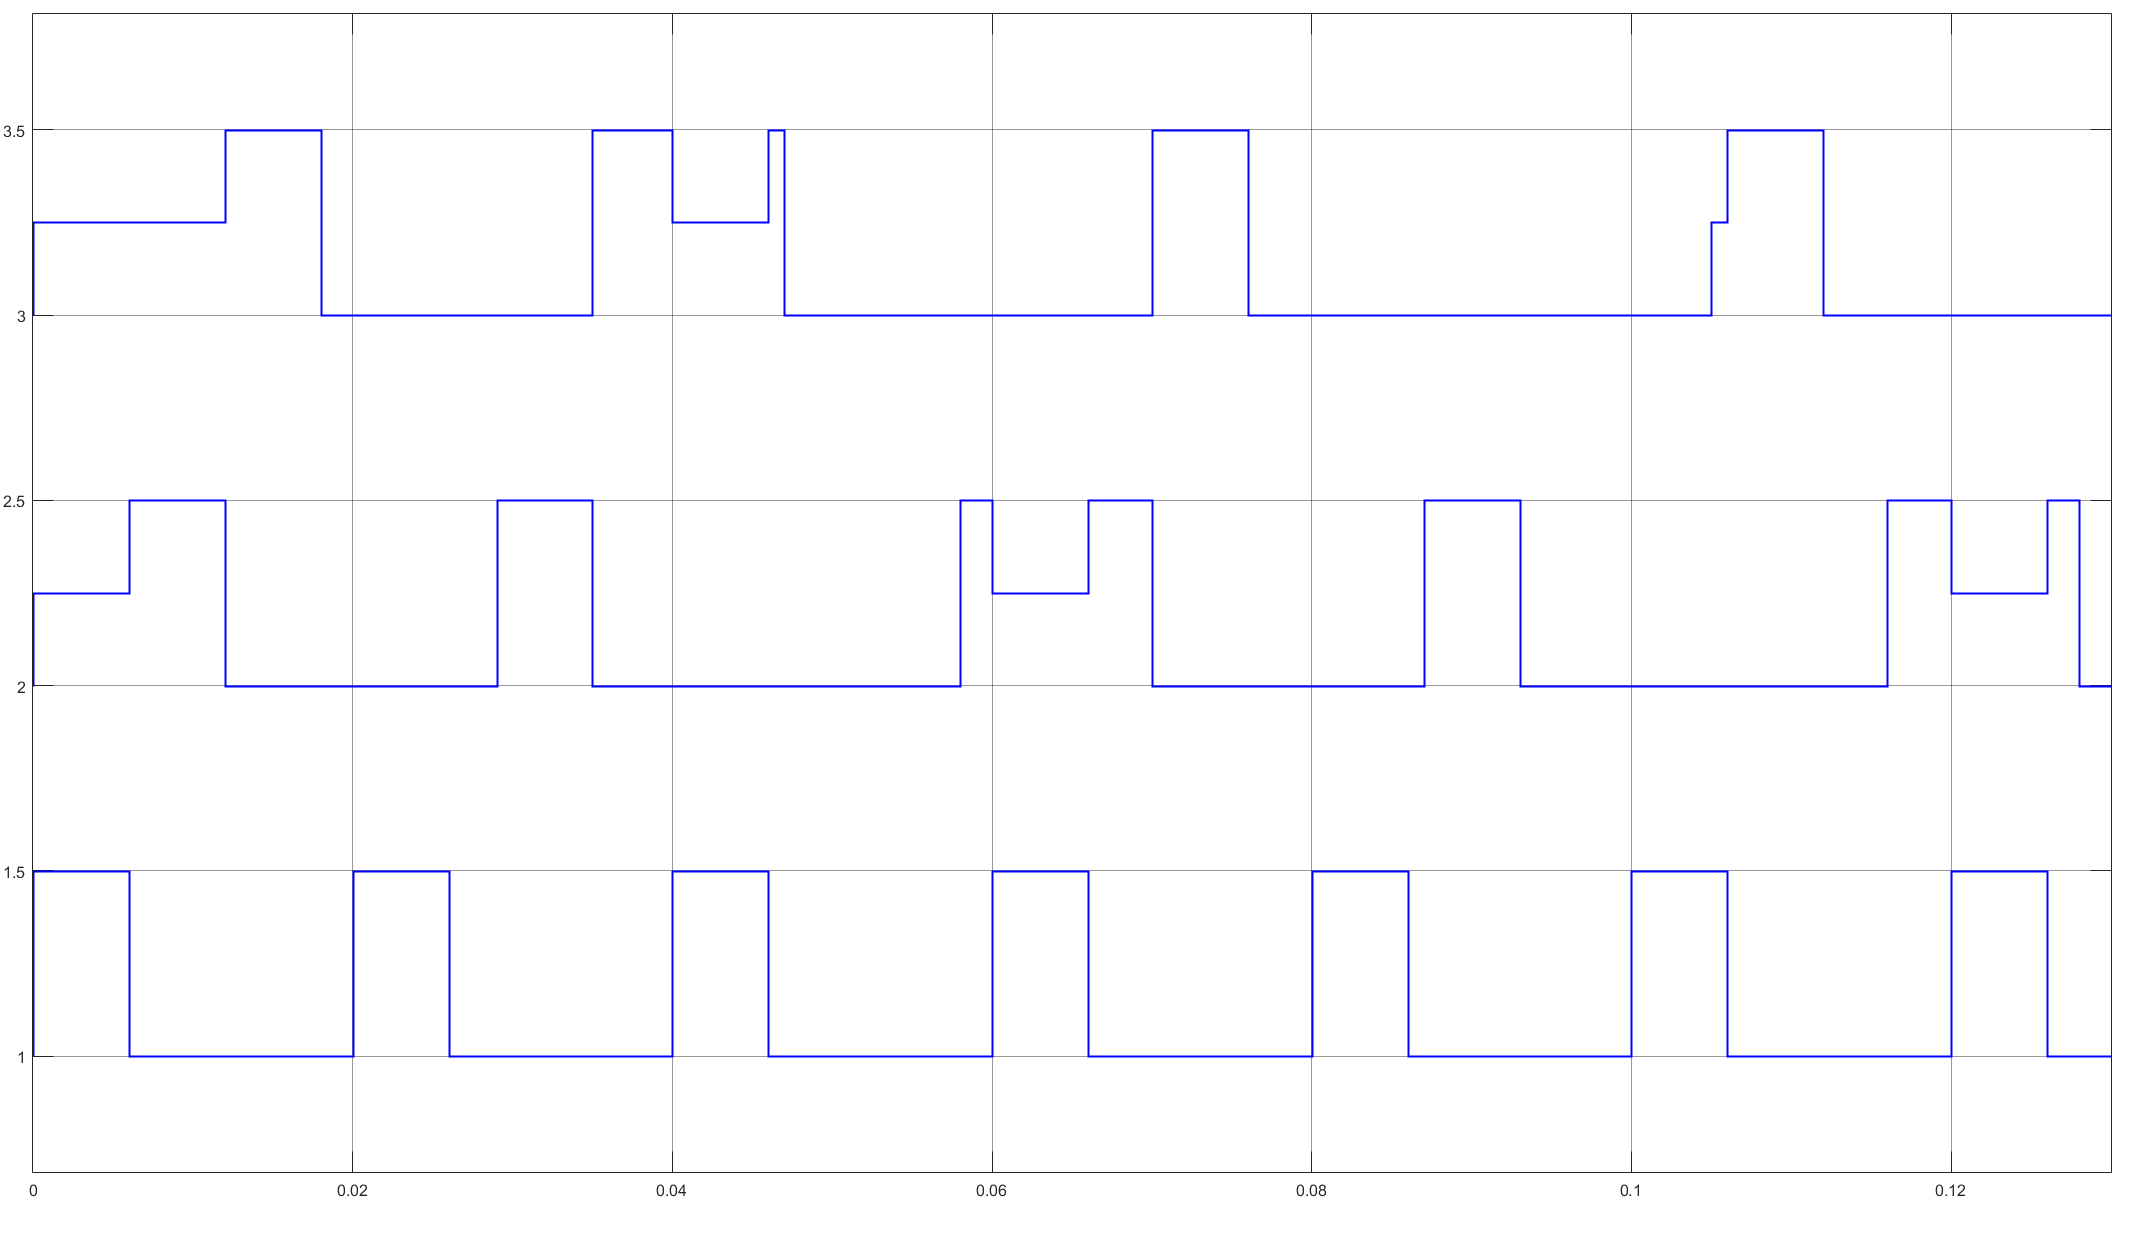
\includegraphics[scale=0.2]{ex42.png}
      \caption{Schedule from Simulink for 6 ms}
        \label{fig:ex32}
      \end{figure}
    \end{center}


\subsection{} %5
The longest pendulum becomes unstable after a few seconds due to missed deadlines.
\begin{center}
      \begin{figure}[H]
      \centering
        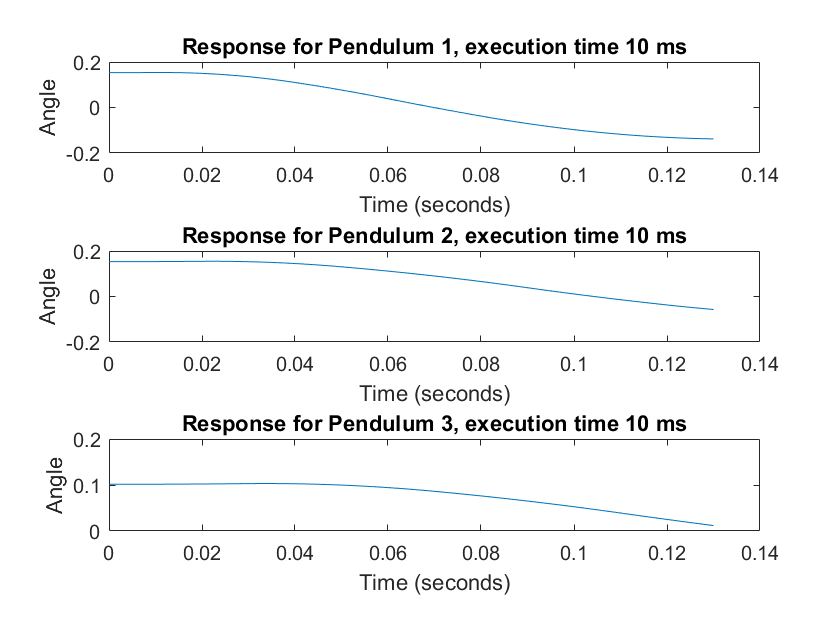
\includegraphics[scale=0.5]{ex531.png}
        \caption{Pendulum angles for the three different pendulums}
        \label{fig:ex31}
      \end{figure}
    \end{center}
    
    \begin{center}
      \begin{figure}[H]
      \centering
        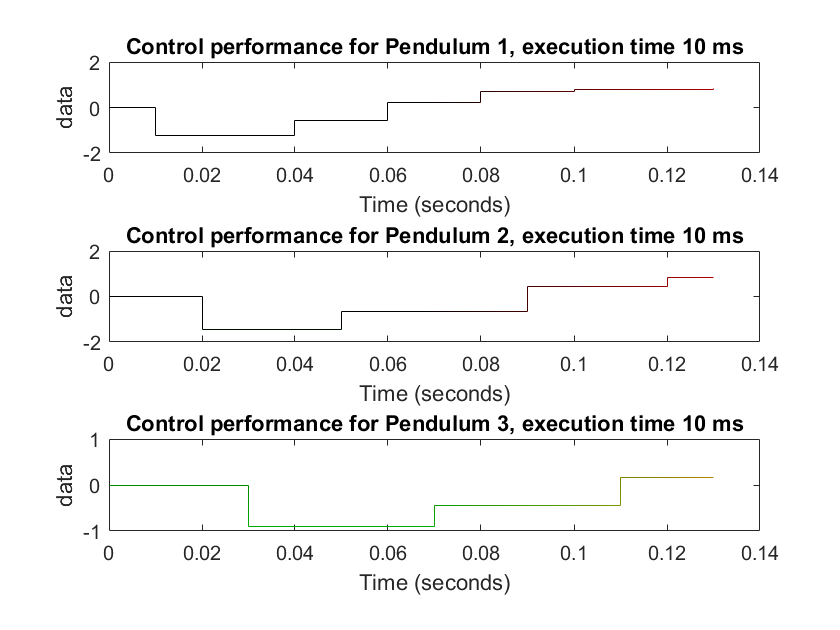
\includegraphics[scale=0.5]{ex532.png}
      \caption{Control signal for pendulum}
        \label{fig:ex32}
      \end{figure}
    \end{center}
    
    
Deadlines are missed for the long pendulum which means that the tasks
are not schedulable. This is verified by calculating the equation
\begin{equation}
 U \le n(2^{(1/n)}-1 = 3*(2^{(1/3)}-1) = 0.779
\end{equation}
where
\begin{equation}
U = \sum\limits_{i=1}^n \frac{C_i}{D_i} = \frac{10}{20}+\frac{10}{29}+\frac{10}{35} = 1.13
\end{equation}
This means that it is not schedulable due to
\begin{equation}
1.13 > 0.779
\end{equation} 
Our schedule for a computation time of 10 ms can be seen in figure
\ref{fig:ex541} as well can the schedule from Simulink be seen in figure
\ref{fig:ex542}. Our schedule is equal to the one from Simulink.
\begin{center}
	\begin{figure}[H]
      \centering
	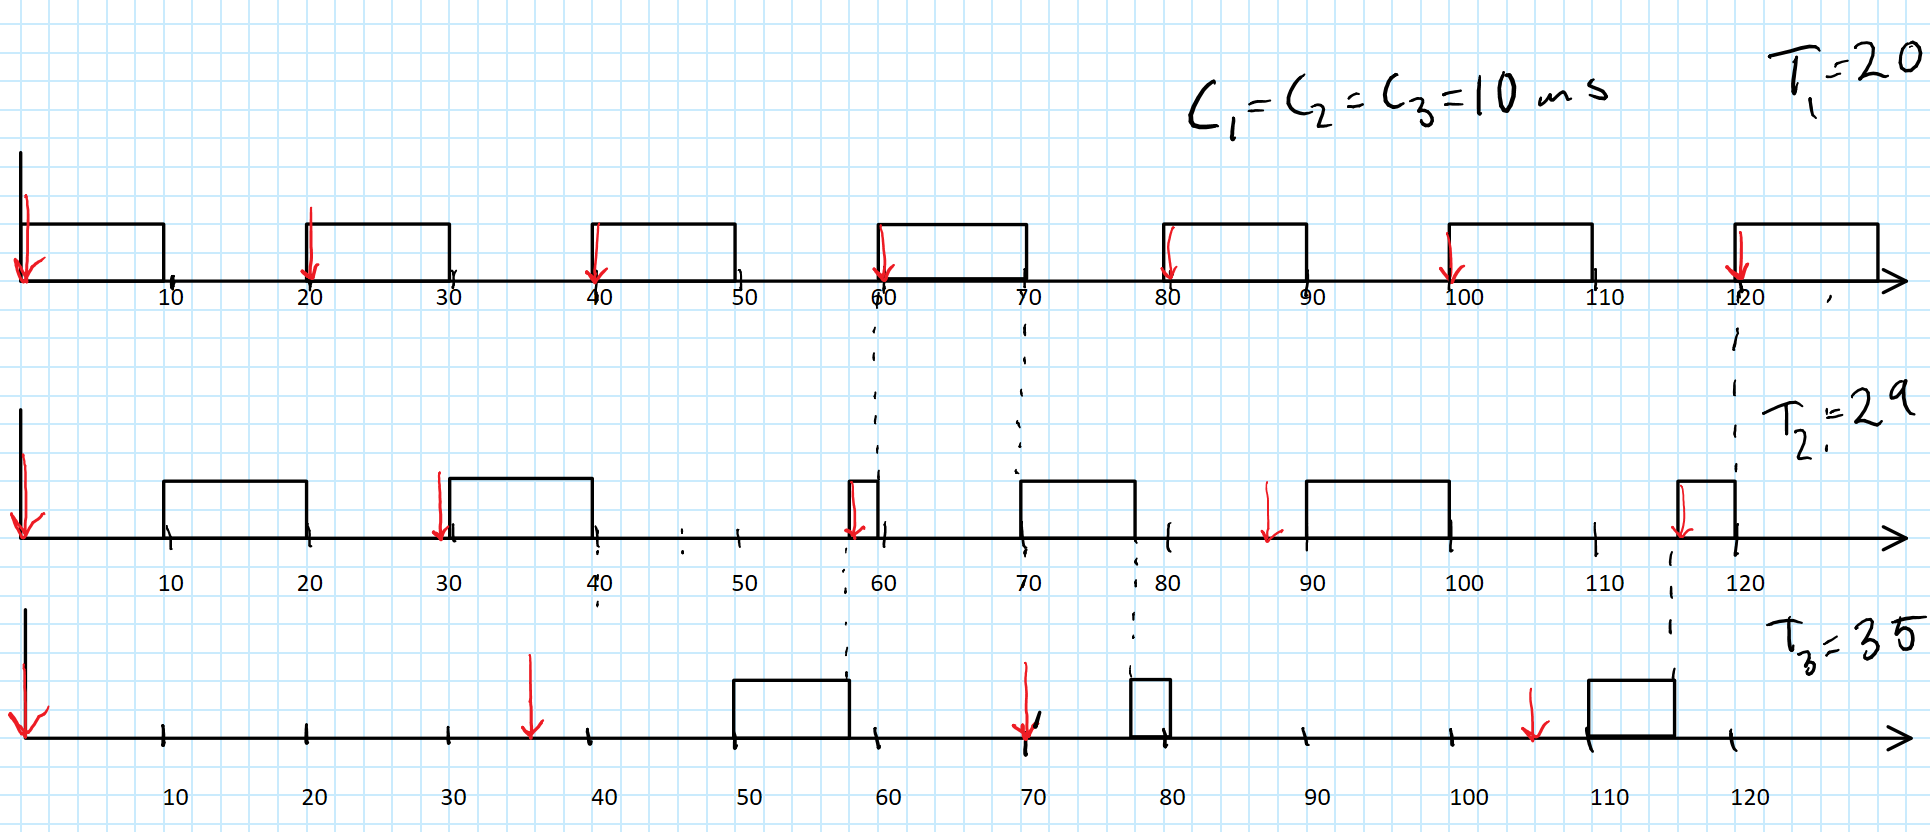
\includegraphics[scale=0.3]{ex541.png}
	\caption{Our schedule for 10 ms computation time}
	\label{fig:ex541}
	\end{figure}
\end{center}
\begin{center}
	\begin{figure}[H]
      \centering
	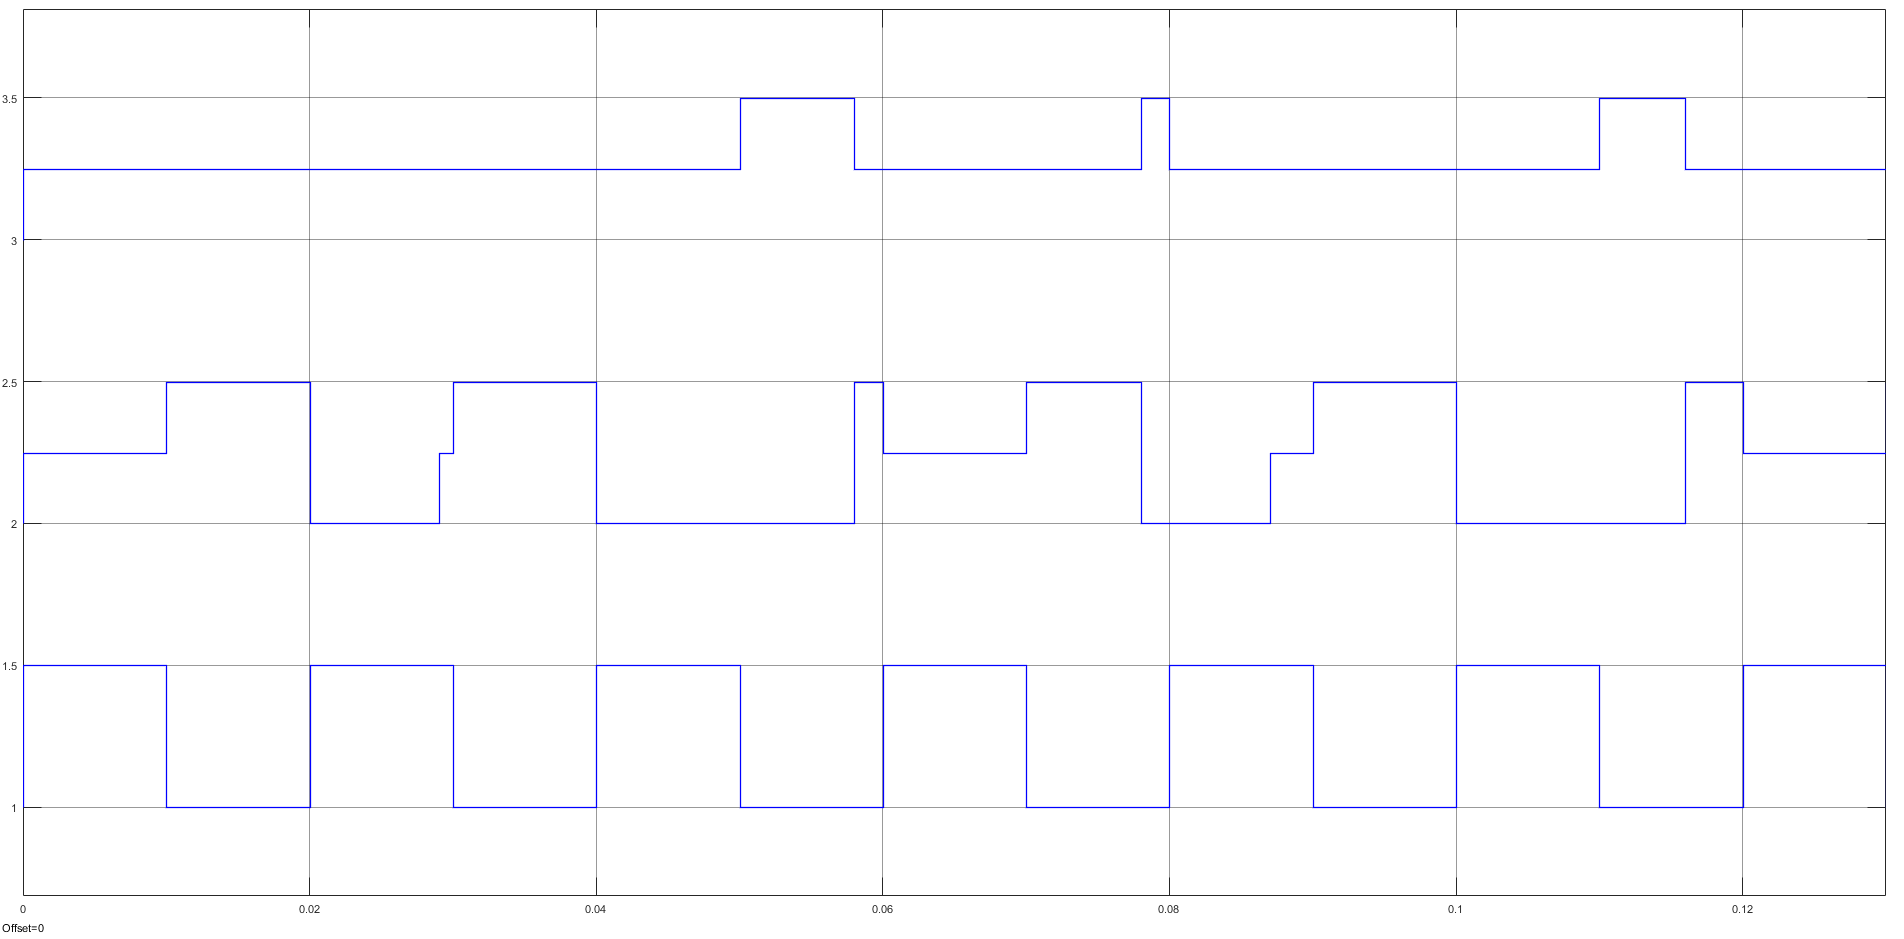
\includegraphics[scale=0.2]{ex542.png}
	\caption{Simulink schedule for 10 ms computation time}
	\label{fig:ex542}
	\end{figure}
\end{center}


%%%%%%%%%%%%%%%%%%%%%%%%%%%%%%%%%%%% TASK 1.2 %%%%%%%%%%%%%%%%%%%%%%%%%%%%

\section{Earliest Deadline First}
\subsection{}
Earliest deadline first scheduling executes the task with the shortest
time left of its deadline $d_k$. This means that the schedule
dynamically changes depending on the different task's deadlines. The
advantages of EDF compared to RM is that EDF fully uses the processor
computational power while RM is limited to $U=n(2^{1/n}-1)$.

\subsection{} %6.2
Tasks are schedulable with \textbf{Earliest Deadline First} if 
\begin{equation}
U \le 1
\end{equation}
which in this case is
\begin{equation}
  U = \frac{6}{20}+\frac{6}{29}+\frac{6}{35}=0.678 < 1
\end{equation}
This means that the tasks are schedulable which we verified with our schedule that is shown in 2.4.
\subsection{} %6.3
The pendulums have stabilized. The shortest one is the hardest to
control just as with Rate monotonic scheduling. There is not a huge
difference in the control signal but you can see the sampling time
differences. Since pendulum 3 is sampled the slowest it also takes
longest time for it to be completely stable.
\begin{center}
	\begin{figure}[H]
      \centering
	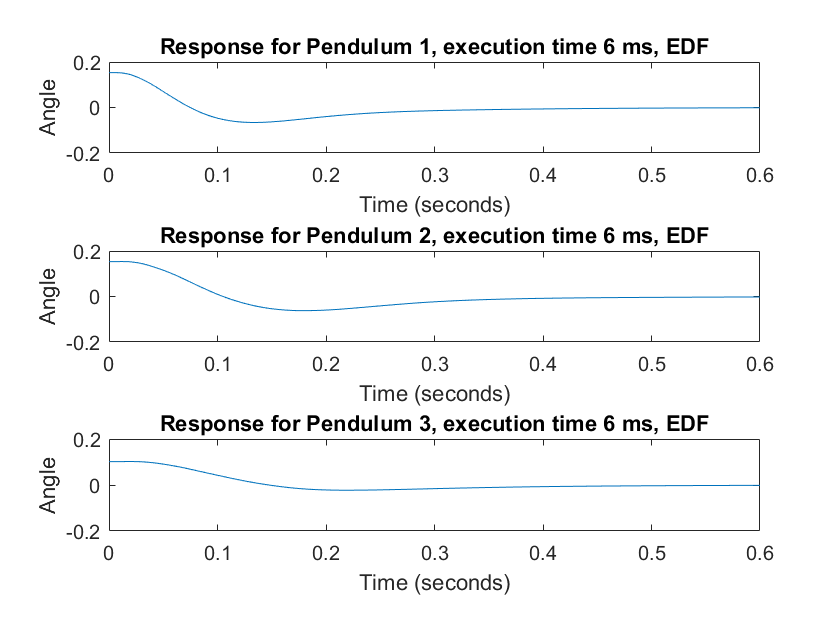
\includegraphics[scale=0.5]{ex61.png}
	\caption{Pendulum angles for the three different pendulums}
	\label{fig:ex61}
	\end{figure}
\end{center}
\begin{center}
	\begin{figure}[H]
      \centering
	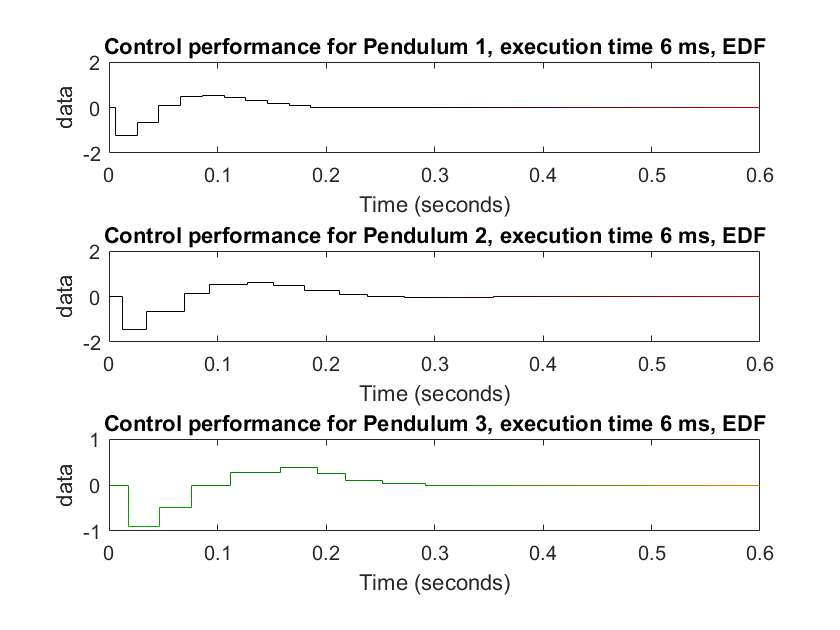
\includegraphics[scale=0.5]{ex62.png}
	\caption{Control signal  for the three different pendulums}
	\label{fig:ex62}
	\end{figure}
\end{center}

\subsection{} 
Our schedule for EDF with 6 ms can be seen in figure \ref{fig:ex641}. The
schedule from Simulink can be seen in figure \ref{fig:ex642}. The result from
Simulink agrees with our schedule; all tasks are carried out before the
next sampling time.
\begin{center}
	\begin{figure}[H]
      \centering
	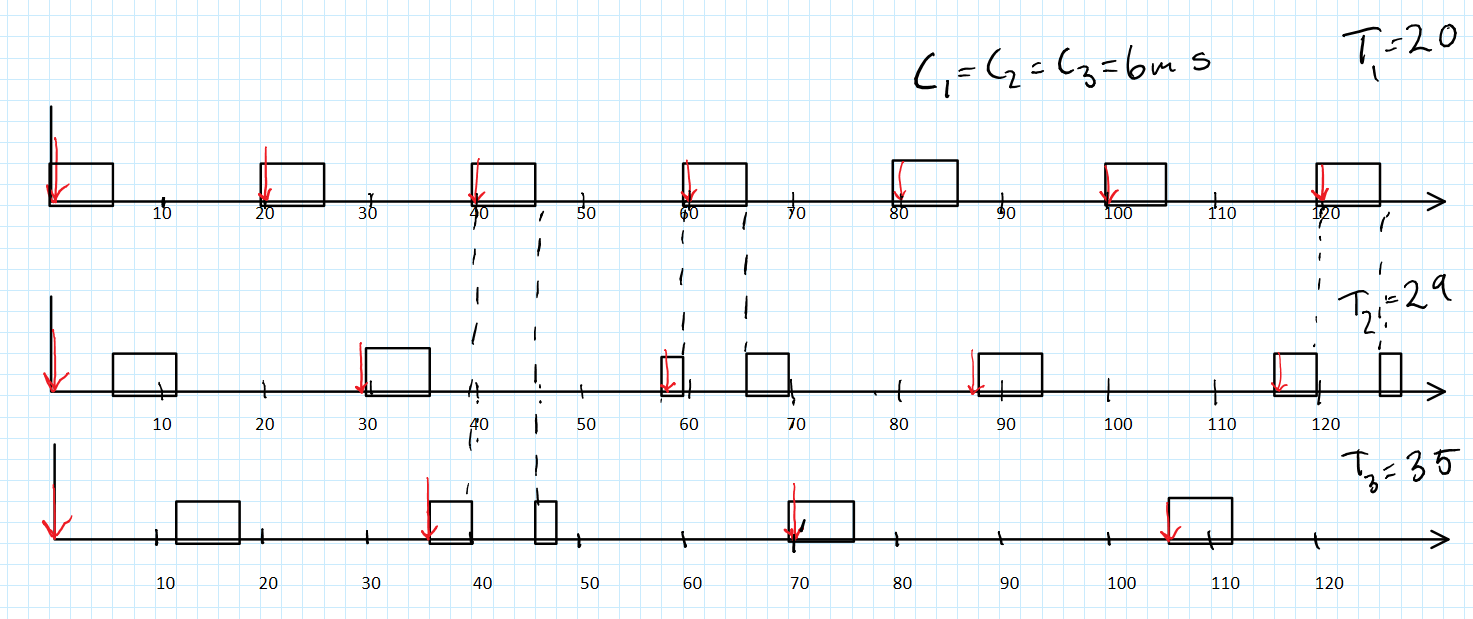
\includegraphics[scale=0.5]{ex641.png}
	\caption{Our schedule for 6 ms computation time, EDF}
	\label{fig:ex641}
	\end{figure}
\end{center}
\begin{center}
	\begin{figure}[H]
      \centering
	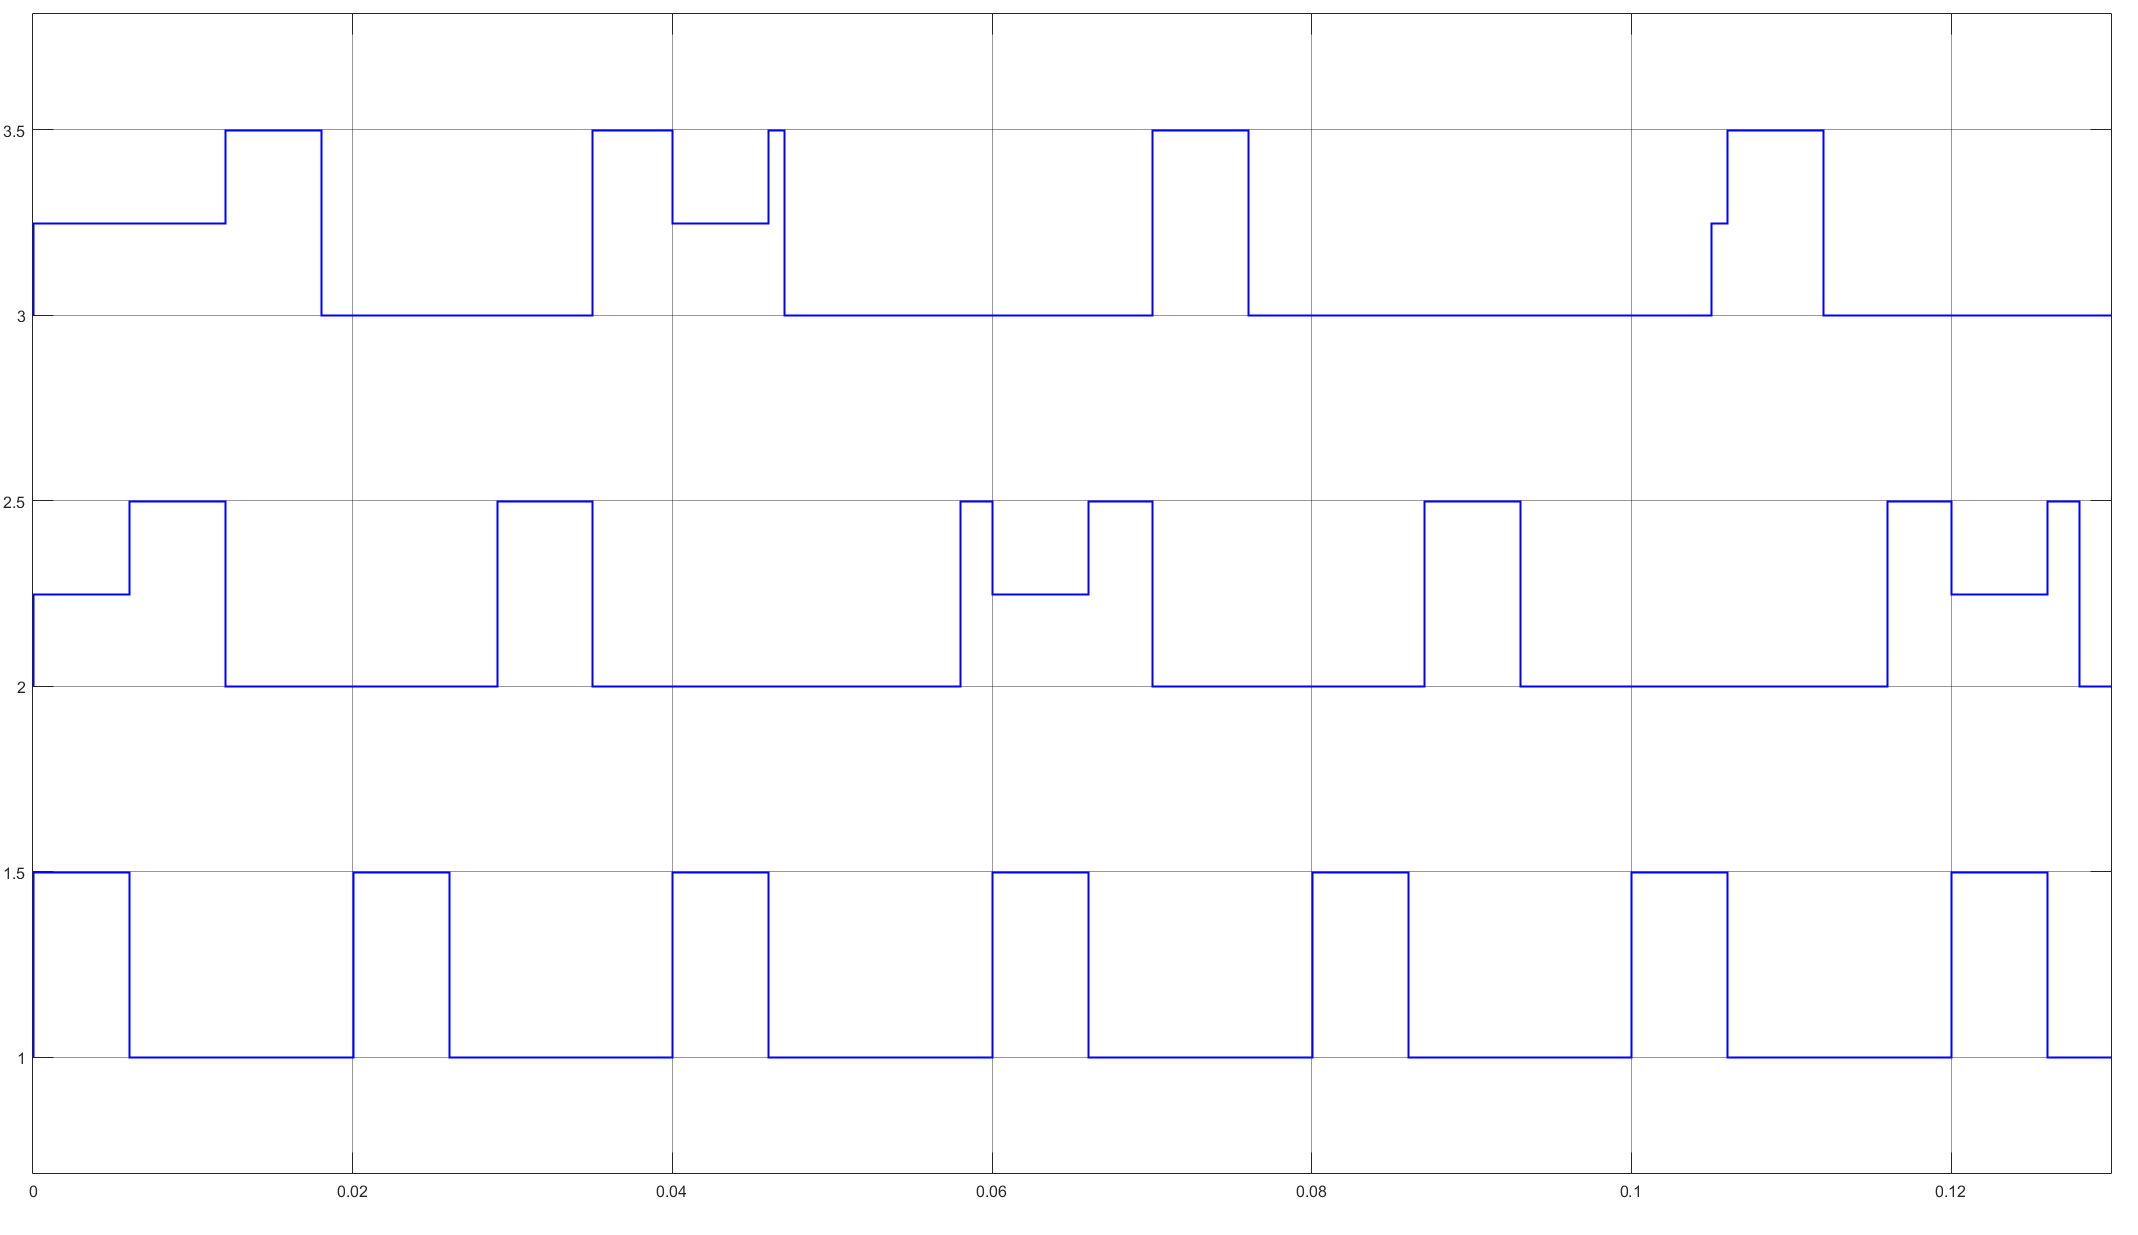
\includegraphics[scale=0.2]{ex642.png}
	\caption{Simulink schedule for 6 ms computation time, EDF}
	\label{fig:ex642}
	\end{figure}
\end{center}

\subsection{}
Even though deadlines are missed with EDF the pendulums still stabilizes. 
\begin{center}
	\begin{figure}[H]
      \centering
	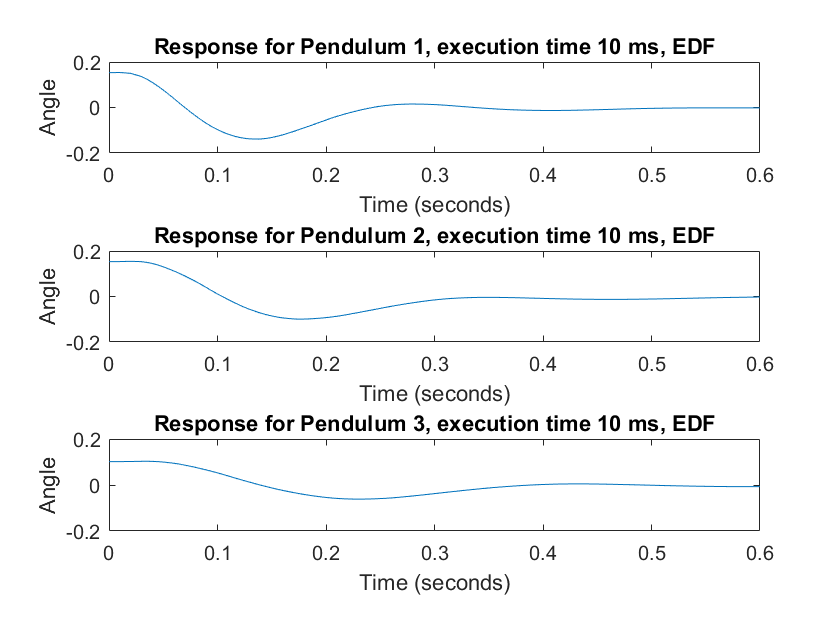
\includegraphics[scale=0.5]{ex6531.png}
	\caption{Pendulum angles for the three different pendulums, EDF}
	\label{fig:ex61}
	\end{figure}
\end{center}
\begin{center}
	\begin{figure}[H]
      \centering
	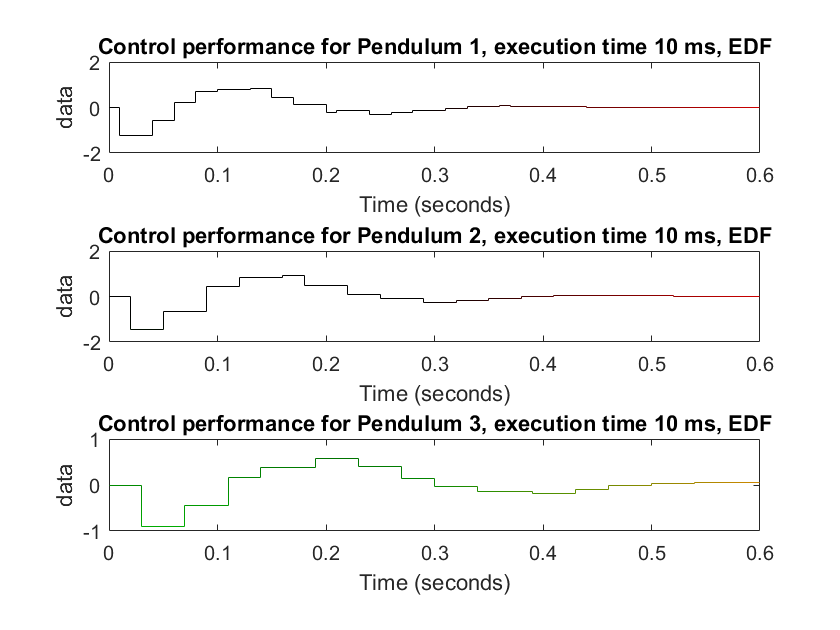
\includegraphics[scale=0.5]{ex6532.png}
	\caption{Control signal  for the three different pendulums, EDF}
	\label{fig:ex62}
	\end{figure}
\end{center}
The tasks are not schedulable with a computation time of 10 ms due to 
\begin{equation}
U = \sum\limits_{i=1}^n \frac{C_i}{D_i} = \frac{10}{20}+\frac{10}{29}+\frac{10}{35} = 1.13 > 1
\end{equation}
which we also verified when we created our schedule. Our schedule for a
computation time of 10 ms with EDF is shown in figure \ref{fig:ex6541}. Simulink
schedule for a computation time of 10 ms is shown in figure
\ref{fig:ex6542}. Our
schedule matches the one from Simulink.

\begin{center}
	\begin{figure}[H]
      \centering
	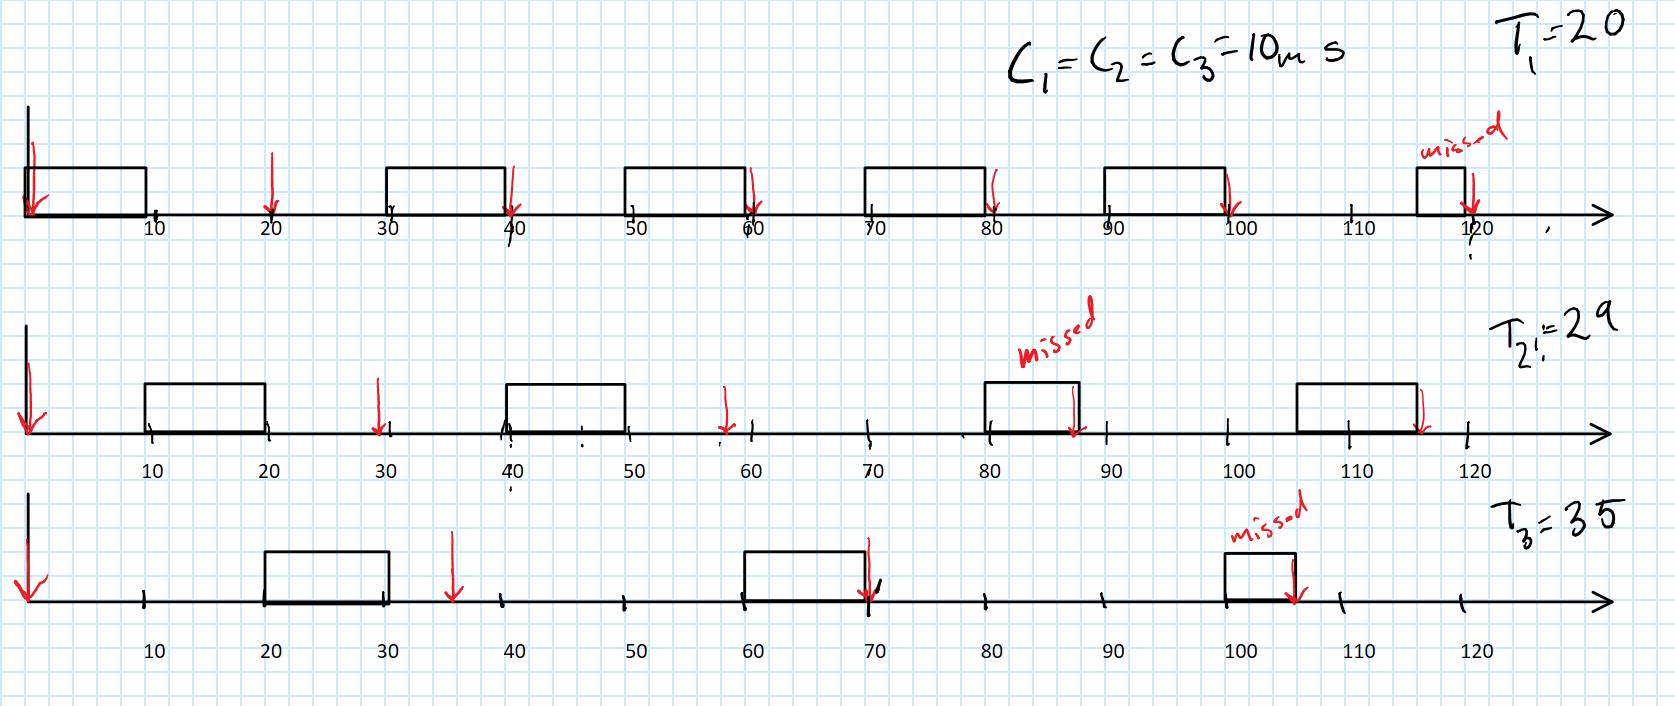
\includegraphics[scale=0.4]{ex6541.png}
	\caption{Our schedule for 10 ms computation time, EDF}
	\label{fig:ex6541}
	\end{figure}
\end{center}
\begin{center}
	\begin{figure}[H]
      \centering
	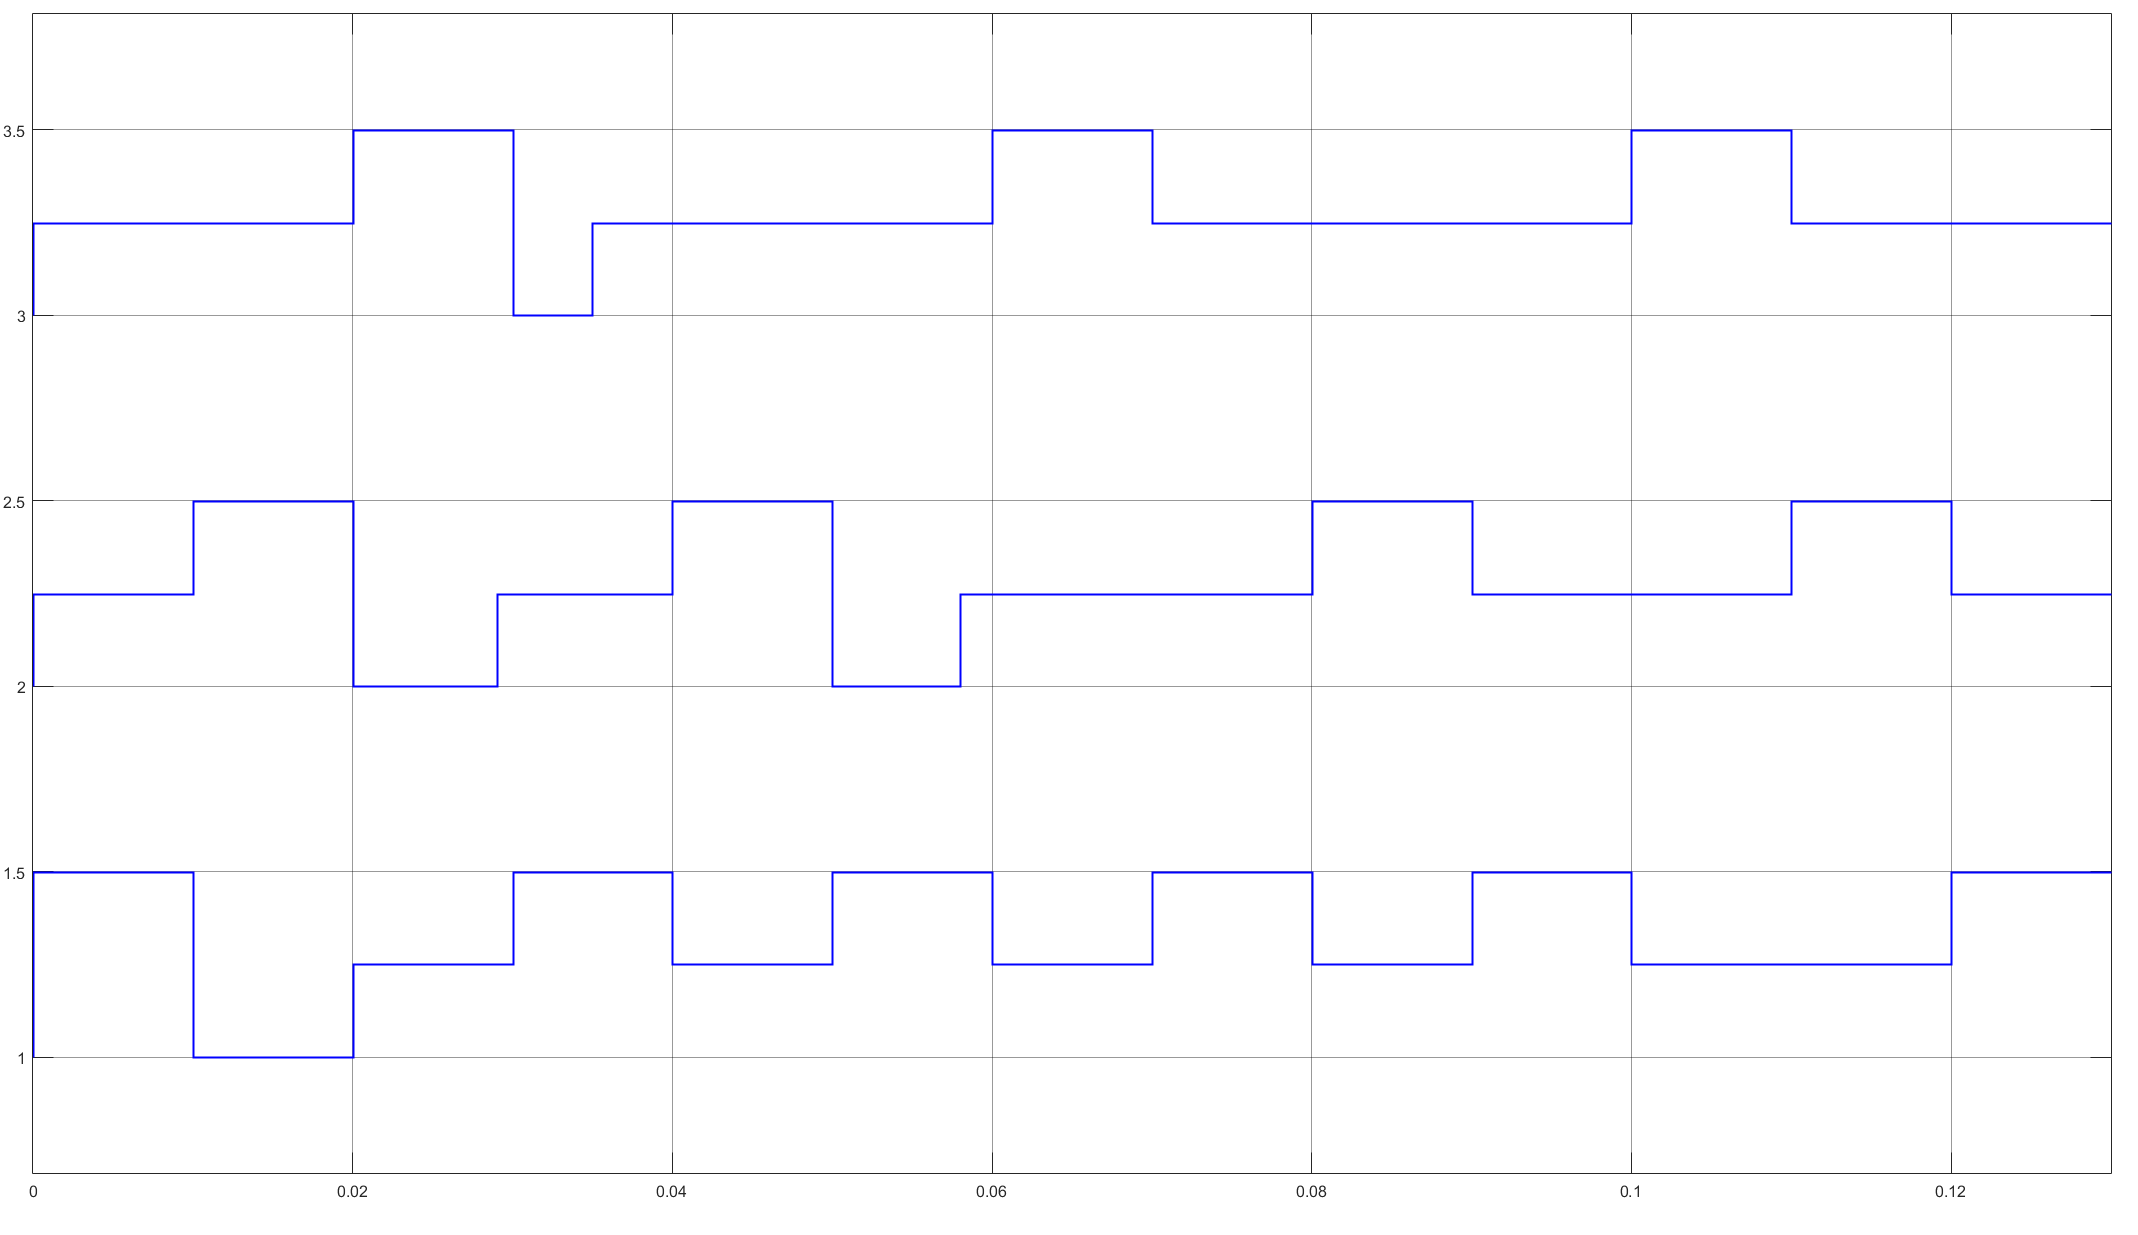
\includegraphics[scale=0.2]{ex6542.png}
	\caption{Simulink schedule for 10 ms computation time, EDF}
	\label{fig:ex6542}
	\end{figure}
\end{center}

\subsection{}
The controller performs better with Earliest Deadline First due to every
pendulum stabilizes which pendulum 3 does not with Rate Monotonic. 



%%%%%%%%%%%%%%%%%%%%%%%%%%%%%%%%%%%% TASK 2 %%%%%%%%%%%%%%%%%%%%%%%%%%%%


\section{Network Control System}
\subsection{} %1
We have the following system
  \begin{equation}
    \dot{x}(t) = Ax(t)+Bu(t) \\
    y(t) = Cx(t)
    \label{eq:system}
  \end{equation}
where
\begin{center}
$A=0$ \\
$B=I$
\end{center}
and the discrete controller
\begin{equation}
    u(kh) = -Kx(kh),    k = 0,1,2,...
    \label{eq:u}
\end{equation}
discretizing the system in equation \ref{eq:system} will give that the
plant can be writen
\begin{equation}
    x((k+1)h)=\Phi x(kh)+\Gamma_{0}(\tau_)u(kh)+\Gamma_{1}(\tau)u((k-1)h)
    \label{eq:disys}
\end{equation}
Given that $A=0, B=I$ and that $\tau = \tau_{sc}+\tau_{ca}\le h$ we can
calculate the matrices,
\begin{align*}
    &\Phi=e^{Ah}=1 \\
    &\Gamma_{0}(\tau)=\int_{0}^{h-\tau}e^{As}Bds=I(h-\tau) \\
    &\Gamma_{1}(\tau)=\int_{h-\tau}^{h}e^{As}Bds=I\tau
\end{align*}
This, together with equation \ref{eq:u} and the system in equation \ref{eq:disys}
gives,
\begin{equation}
  x(kh+\tau)=x(kh)+
  \begin{bmatrix}
    -IK(h-\tau) & I\tau\\
    -K & 0
  \end{bmatrix}
  \begin{bmatrix}
    x(kh) \\
    u(kh+\tau)
  \end{bmatrix}
\end{equation}

\subsection{} % (fold)

Considering the systems denominator of the transfer function on the
form, 
\begin{equation}
    d(z) = z^2+a_1z+a_2,
\end{equation}
the system is BIBO stable if the poles,
\begin{equation}
  p_1,p_2=-\frac{a_2}{2}\pm \sqrt{\frac{a_1^2-4a_2}{4}}.
\end{equation}
This gives us that
\begin{equation}
    a_1=-(p_1+p_2)
    \label{eq:a1}
\end{equation}
\begin{equation}
    a_2=p_1p_2.
    \label{eq:a2}
\end{equation}
For the system to be stable, the poles needs to lie inside the unit
circle, meaning that,
\begin{equation}
    p_1, p_2 < 1.
\end{equation}
With equation \ref{eq:a1} and \ref{eq:a2} we can now form the criteria for stabillity,
\begin{equation}
    |a_2|=|p_1p_2|=|p_1||p_2|<1
    \label{eq:a2l}
\end{equation}
and for $a_1$
\begin{equation}
    |a_1|<1+a_2
    \label{eq:a1l}
\end{equation}
Calculating the eigenvalues of \ref{eq:disys} will give the poles of the
system, which together with equation \ref{eq:a2} and \ref{eq:a1} give,
\begin{equation}
  a_2 = -KI\tau
  \label{eq:a2new}
\end{equation}
and
\begin{equation}
    a_1 = IKh-IK\tau-1
    \label{eq:a1new}
\end{equation}
Combining equation \ref{eq:a1new} and \ref{eq:a2new} with \ref{eq:a2l}
and \ref{eq:a1l} and solving for $\tau/h$ will give us that the
relation,
\begin{equation}
  max\left\{\frac{1}{2}-\frac{1}{KIh},0\right\}<\frac{\tau}{h}<min\left\{\frac{1}{KIh},1\right\}.
\end{equation}
must be satisfied for stability.

The stability criteria can be represented graphically plotted as a
stability region. This can be seen in figure \ref{fig:stabilityRegion}.
\begin{figure}[H]
    \begin{center}
      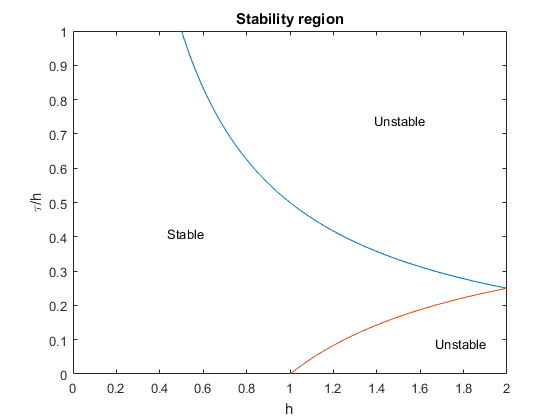
\includegraphics[scale=0.5]{stabilityRegion.png}
      \caption{Stability region}
      \label{fig:stabilityRegion}
    \end{center}
\end{figure}


\subsection{}
The system will become unstable when a delay of 0.4 seconds is used. The settling time for 0.39 is quite long but the system does stabilize. Figure \ref{fig:network_delay} shows different time delay settings in Simulink. It clearly shows that a delay of 0.3 seconds still makes the system stabilize quickly while a delay of 0.4 makes it unstable.

\begin{center}
      \begin{figure}[H]
      \centering
        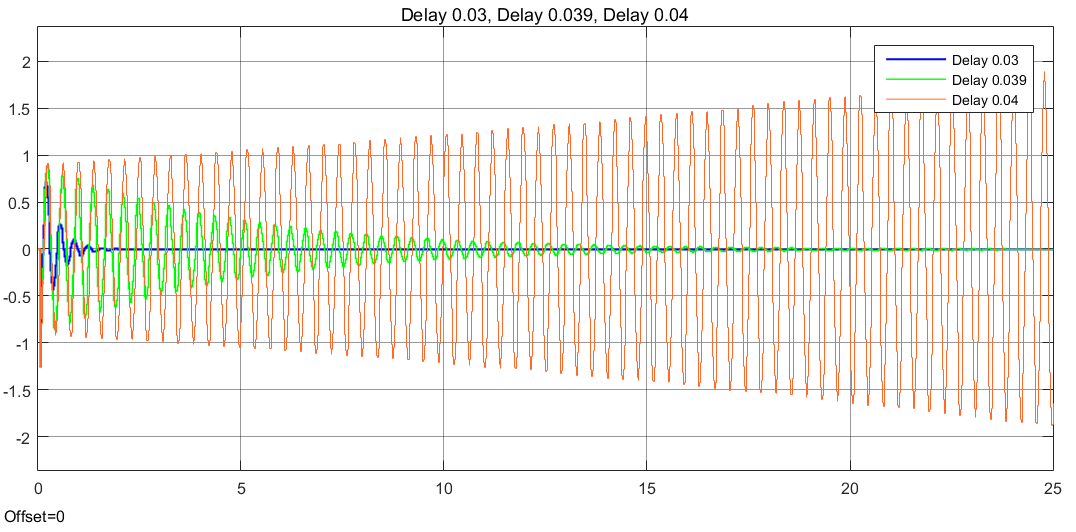
\includegraphics[scale=0.5]{network_delay.png}
        
      \caption{Control signal for different delay settings}
      \label{fig:network_delay}
      
      \end{figure}
    \end{center}
    

% subsection  (end)

%%%%%%%%%%%%%%%%%%%%%%%%%%%%%%%%%%%% TASK 3 %%%%%%%%%%%%%%%%%%%%%%%%%%%%

\section{Discrete Event System}
\subsection{}
Since the state machines M1 and M2 have the same states they are
represented as the same state machine. This can be seen in Figure 17.	
\begin{center}
	\begin{figure}[H]
      \centering
	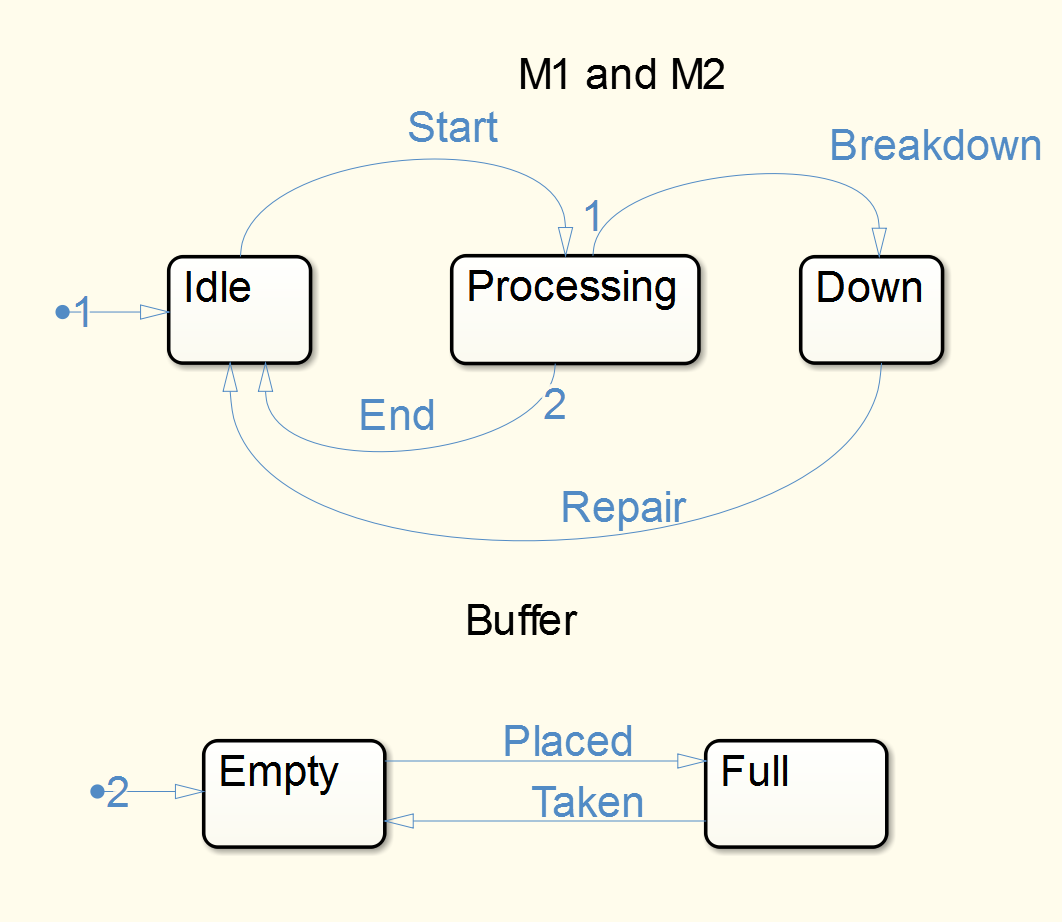
\includegraphics[scale=0.5]{des1.png}
	\label{fig:des1}
	\caption{State machine for M1, M2 and the buffer}
	\end{figure}
\end{center}

\subsection{}
Each state in Figure 18 represents the current state in M1, M2 and the
buffer. There are 18 different states available 
\begin{equation}
3^2*2 = 18
\end{equation}
since both machines has 3 states and the buffer has 2.
The form ${x,y,z}$ is used where $x=M1,y=Buffer,z=M2$. For example
\begin{center}
$IEI = {Idle,Empty,Idle}$
\end{center}
The events of each transition are not shown in Figure 18 due to too many
transitions and the events are obvious.
\begin{center}
	\begin{figure}[H]
      \centering
	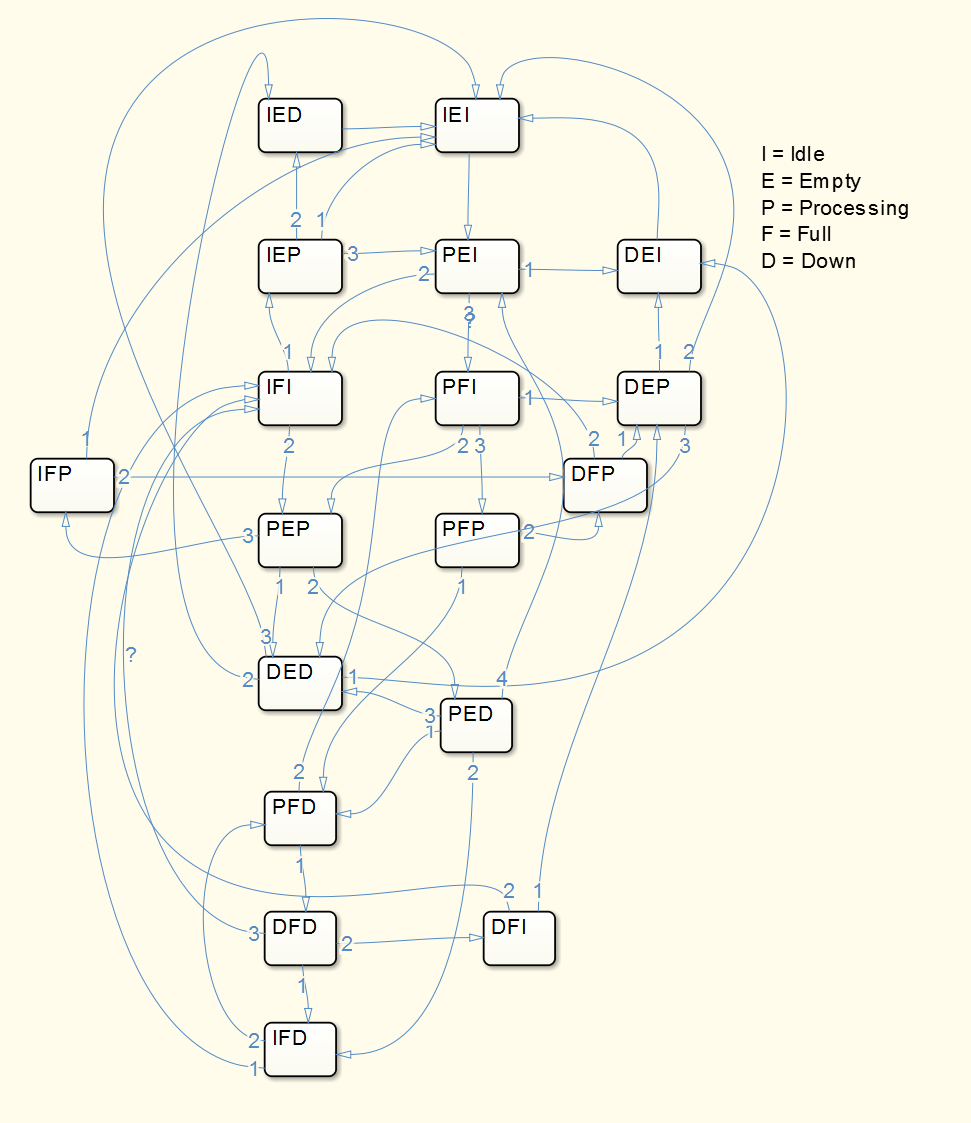
\includegraphics[scale=0.7]{des2.png}
	\label{fig:des1}
	\caption{State machine for M1, M2 and the buffer}
	\end{figure}
\end{center}

\subsection{}
With the requirements given some states could be disregarded due to our
interpretation of the functionality of the state machine. We assume that
when a process has finished a product and put it in the buffer it goes
to idle due to a new product can't begin processing if the buffer is
full even though it still could be in the processing state.
\begin{center}
	\begin{figure}[H]
      \centering
	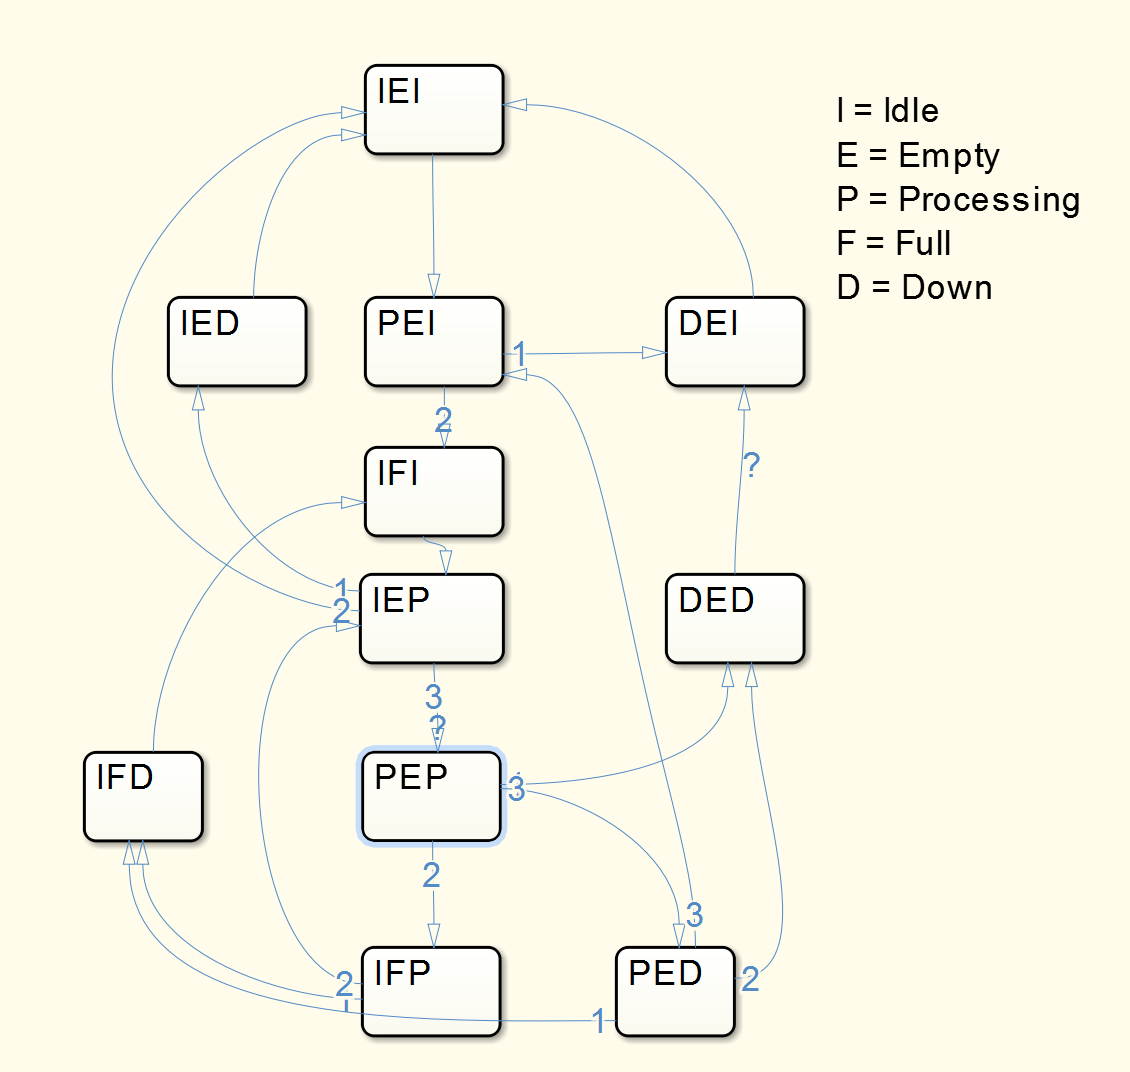
\includegraphics[scale=0.5]{des3.png}
	\label{fig:des1}
	\caption{State machine for M1, M2 and the buffer}
	\end{figure}
\end{center}

\subsection{}
A controller to make sure the requirements are fulfilled when using the
complete Discrete Event System from 4.2 needs to have information of
which state each machine is in. Then by using that information
\emph{Guards} can be used on each transition along with the event to
ensure it goes to the right state. A \emph{Guard} is a form of
If-statement used in state machines to set requirements for transitions.

\end{document}
